\documentclass{jarticle}
\usepackage[top=20truemm,bottom=15truemm,left=20truemm,right=20truemm]{geometry}
\usepackage{jlisting, listings, here}
\usepackage[dvipdfmx]{graphicx}
\makeatletter
\def\maketitle{%
\null
\thispagestyle{empty}%
\vfill
\begin{center}\leavevmode
\normalfont
{\LARGE \@title\par}%
\vskip 1cm
{\Large \@author\par}%
\vskip 1cm
{\Large \@date\par}%
\end{center}%
\vfill
\null
\@thanks%\vfil\null
\cleardoublepage
}
\makeatother
\lstset{language=c,
basicstyle=\ttfamily\scriptsize,
commentstyle=\textit,
classoffset=1,
keywordstyle=\bfseries,
frame=tRBl,
framesep=5pt,
showstringspaces=false,
stepnumber=1,
numberstyle=\tiny,
tabsize=2,
numbers = left,
stepnumber=1
}
\title{ソフトウェア演習V 課題2(再々提出)}
\author{15122013 尾持涼介}
\date{提出日:2018年2月9日}

\begin{document}
\maketitle

\section{作成したプログラムの設計情報}
\subsection{全体構成}
各ファイルで記述した関数は以下の通りである。
\begin{itemize}
  \item main.c
  \begin{itemize}
    \item main関数
    \item void error(char *mes)
  \end{itemize}
  \item scan.c
  \begin{itemize}
    \item int keyword\_search(char *string)
    \item int init\_scan(char *filename)
    \item int keyword\_search(char *string)
    \item int scan()
    \item int get\_linenum()
    \item void end\_scan()
  \end{itemize}
  \item prettyprinter.c
  \begin{itemize}
    \item int parse\_program()
    \item int block()
    \item int var\_decl()
    \item int var\_names()
    \item int type()
    \item int ar\_type()
    \item int sub\_decl()
    \item int form\_para()
    \item int fukugou()
    \item int statement()
    \item int bunki()
    \item int kurikaeshi()
    \item int call\_st()
    \item int exp\_narabi()
    \item int dainyu()
    \item int var()
    \item int shiki()
    \item int simple()
    \item int kou()
    \item int inshi()
    \item int input\_st()
    \item int output\_st()
    \item int shitei()
    \item void indent()
  \end{itemize}
\end{itemize}

次に、各関数の呼び出し関係、データ参照関係について述べる。
\begin{itemize}
  \item main.c
  \begin{itemize}
    \item main関数内
    \begin{itemize}
      \item init\_scan()関数を呼び出し
      \item scan()関数を呼び出し
      \item parse\_program()関数を呼び出し
      \item end\_scan()関数を呼び出し
    \end{itemize}
    \item error関数内
    \begin{itemize}
      \item get\_linenum()関数を参照
    \end{itemize}
  \end{itemize}
  \item scan.c
  \begin{itemize}
    \item scan()関数内
    \begin{itemize}
      \item keyword\_search()関数を呼び出し
    \end{itemize}
  \end{itemize}
  \item prettyprinter.c
  \begin{itemize}
    \item parse\_program()関数内
    \begin{itemize}
      \item scan()関数を呼び出し
      \item block()関数を呼び出し
    \end{itemize}
    \item block()関数内
    \begin{itemize}
      \item var\_decl()関数を呼び出し
      \item sub\_decl()関数を呼び出し
      \item fukugou()関数を呼び出し
    \end{itemize}
    \item var\_decl()関数内
    \begin{itemize}
      \item indent()関数を呼び出し
      \item scan()関数を呼び出し
      \item var\_names()関数を呼び出し
      \item type()関数を呼び出し
    \end{itemize}
    \item var\_names()関数内
    \begin{itemize}
      \item scan()関数を呼び出し
      \item ar\_types()関数を呼び出し
    \end{itemize}
    \item ar\_types()関数内
    \begin{itemize}
      \item scan()関数を呼び出し
    \end{itemize}
    \item sub\_decl()関数内
    \begin{itemize}
      \item indent()関数を呼び出し
      \item scan()関数を呼び出し
      \item form\_para()関数を呼び出し
      \item var\_decl()関数を呼び出し
      \item fukugou()関数を呼び出し
    \end{itemize}
    \item form\_para()関数内
    \begin{itemize}
      \item scan()関数を呼び出し
      \item var\_names()関数を呼び出し
      \item type()関数を呼び出し
    \end{itemize}
    \item fukugou()関数内
    \begin{itemize}
      \item scan()関数を呼び出し
      \item statement()関数を呼び出し
      \item indent()関数を呼び出し
    \end{itemize}
    \item statemen()関数内
    \begin{itemize}
      \item indent()関数を呼び出し
      \item dainyu()関数を呼び出し
      \item bunki()関数を呼び出し
      \item kurikaeshi()関数を呼び出し
      \item scan()関数を呼び出し
      \item call\_st()関数を呼び出し
      \item input\_st()関数を呼び出し
      \item output\_st()関数を呼び出し
      \item fukugou()関数を呼び出し
    \end{itemize}
    \item bunki()関数内
    \begin{itemize}
      \item scan()関数を呼び出し
      \item shiki()関数を呼び出し
      \item statement()関数を呼び出し
      \item indent()関数を呼び出し
    \end{itemize}
    \item kurikaeshi()関数内
    \begin{itemize}
      \item scan()関数を呼び出し
      \item shiki()関数を呼び出し
      \item statement()関数を呼び出し
    \end{itemize}
    \item call\_st()関数内
    \begin{itemize}
      \item scan()関数を呼び出し
      \item exp\_narabi()関数を呼び出し
    \end{itemize}
    \item dainyu()関数内
    \begin{itemize}
      \item var()関数を呼び出し
      \item scan()関数を呼び出し
      \item shiki()関数を呼び出し
    \end{itemize}
    \item var()関数内
    \begin{itemize}
      \item scan()関数を呼び出し
      \item shiki()関数を呼び出し
    \end{itemize}
    \item shiki()関数内
    \begin{itemize}
      \item simple()関数を呼び出し
      \item scan()関数を呼び出し
    \end{itemize}
    \item simple()関数内
    \begin{itemize}
      \item kou()関数を呼び出し
      \item scan()関数を呼び出し
    \end{itemize}
    \item kou()関数内
    \begin{itemize}
      \item inshi()関数を呼び出し
      \item scan()関数を呼び出し
    \end{itemize}
    \item inshi()関数内
    \begin{itemize}
      \item var()関数を呼び出し
      \item scan()関数を呼び出し
      \item shiki()関数を呼び出し
      \item inshi()関数を呼び出し
    \end{itemize}
    \item input\_st()関数内
    \begin{itemize}
      \item scan()関数を呼び出し
      \item var()関数を呼び出し
    \end{itemize}
    \item output\_st()関数内
    \begin{itemize}
      \item scan()関数を呼び出し
      \item shitei()関数を呼び出し
    \end{itemize}
    \item shitei()関数内
    \begin{itemize}
      \item scan()関数を呼び出し
      \item shiki()関数を呼び出し
    \end{itemize}
  \end{itemize}
\end{itemize}
\subsection{各モジュールごとの構成}
prettyprinter.cでは、読み込んだトークンを出力するために次の図\ref{code:token}のような配列を用意した。
\begin{figure}[H]
\begin{center}
\begin{lstlisting}
char *token_str[NUMOFTOKEN+1] = {
"", "",
"program", "var", "array", "of", "begin", "end", "if", "then",
"else", "procedure", "return", "call", "while", "do", "not", "or",
"div", "and", "char", "integer", "boolean", "readln", "writeln", "true",
"false", "", "", "+", "-", "*", "=", "<>", "<", "<=", ">",
">=", "(", ")", "[", "]", ":=", ".", ",", ":", ";", "read","write", "break"
};
\end{lstlisting}
\caption{読み込んだトークンを出力するための配列}
\label{code:token}
\end{center}
\end{figure}
なお、読み込んだトークンが「名前」、「符号なし整数」、「文字列」のときはその実体を出力しなければならないためこの配列は用いない。
そのためそれらのトークンコード1、27、28にあたる要素には何も入れられていない。

また、与えられたマクロ構文に沿ってprettyprinter.c内で関数を定義してif文やwhile文、switch文で判別し、判別したトークンを
適宜出力している。なお、トークンの読み込みにはそれぞれの関数内でscan()関数を呼び出すことにより行っている。また、読み込んだ
トークンの出力はそのトークンが「名前」、「文字列」の時にはstring\_attrを、「符号なし整数」のときはnum\_attrを、それ以外のときは
上記で述べたtoken\_strを参照している。

次に使用した大域変数とその意味について述べる。

\begin{itemize}
  \item main.c内
  \begin{itemize}
    \item int
    numtoken[NUMOFTOKEN+1]:各トークンを数え上げるために使用。各トークンのトークンコードと同じ場所にその個数を格納する。すなわち、例えば、
    numtoken[1]には名前の個数が格納される。なお、NUMOFTOKENとは定義したトークンの個数であり、49と定義されている。
    \item char *tokenstr[NUMOFTOKEN+1] :各トークン名が格納されている。
    \item int token:読み込んだトークンのトークン番号が格納されている。
  \end{itemize}
  \item scan.c内
  \begin{itemize}
    \item int cbuf:ファイルから読み込んだ文字を格納する1文字分の文字バッファ
    \item int line\_cnt:行数を数え上げる変数
    \item int newline:次の文字から新しい行が始まる場合は0、そうでない場合は1を格納しておく。
    \item FILE *fp:ファイルを操作するためのポインタ
    \item char
    string\_attr[MAXSTRSIZE]:読み込んだトークンが「文字列」か「名前」のときにその実体が格納される。なお、MAXSTRSIZEは定義された文字列の最大長であり、1024である。
    \item int num\_attr:読み込んだトークンが「符号なし整数」の時にその実態が格納される。
  \end{itemize}
  \item prettyprinter.c内
  \begin{itemize}
    \item int indentnum:段付け(インデント)をする回数を格納する。
    \item char *token\_str[NUMOFTOKEN+1]:字句を格納する配列。
  \end{itemize}
\end{itemize}

次に各関数内で定義した変数とその意味について述べる

\begin{itemize}
  \item scan.c
  \begin{itemize}
    \item ikeyword\_search()関数内:課題1で記載済み
    \item scan()関数内
    \begin{itemize}
      \item int i:課題1で記載済み
    \end{itemize}
  \end{itemize}
  \item prettyprinter.c
  \begin{itemize}
    \item bunki()関数内
    \begin{itemize}
      \item int flag:分岐文内に複合文があるかどうかを示す変数。(1ならある、0ならない)
    \end{itemize}
    \item kurikaeshi()関数内
    \begin{itemize}
      \item
      int
      flag:繰り返し文内に複合文があるかどうかを示す変数。(1ならある、0ならない)
    \end{itemize}
    \item indent()関数内
    \begin{itemize}
      \item int i:for文によるループで用いる変数。
    \end{itemize}
  \end{itemize}
\end{itemize}
\subsection{各関数の外部(入出力)仕様}
ここでは、各関数の機能、引数と返り値等について説明する。
\subsubsection{main.c内で記述されている関数}
\begin{itemize}
  \item main関数
  \begin{description}
\item[引数]コマンドライン引数としてint ncとchar
*np[]を指定する。ncは指定された引数の個数を表し、npはプログラムを起動するときに指定する引数であり、本プログラムでは読み込むファイル名を指定する。
\item[返り値]プログラムが終了した際に0を返す。
\item[参照・変更する大域変数]なし
\end{description}
\item void error(char *mes)
\begin{description}
\item[機能]エラーが発生したときに、その部分までのプリティプリントをして、エラーメッセージとエラー発生箇所を表示する。
\item[引数]char *mes:表示するエラーメッセージ
\item[返り値]なし
\item[参照・変更する大域変数]なし
\end{description}
\end{itemize}
\subsubsection{scan.c内で記述されている関数}
\begin{itemize}
  \item int init\_scan(char *filename):課題1で記載済み
  \item int keyword\_search(char *string):課題1で記載済み
  \item int scan()
  \begin{description}
\item[機能]トークンを1つスキャンし、そのトークンを識別する。
\item[引数]なし
\item[返り値]トークンのコードを返す。End-of-Fileが現れたときやエラーが発生したときは-1を返す。
\item[参照する大域変数]cbuf、newline、fp
\item[変更する大域変数]cbuf、newline、line\_cnt、num\_attr、string\_attr
\end{description}
\item int get\_linenum():課題1で記載済み
\item void end\_scan():課題1で記載済み
\end{itemize}
\subsubsection{prettyprinter.c内で記述した関数}
なお、以下でNORMALとERRORはそれぞれprettyprinter.c内で0、1と定義されている。
\begin{itemize}
  \item int parse\_program()
  \begin{description}
\item[機能]プログラムを解析する関数
\item[引数]なし
\item[返り値]エラーがあればERRORを、なければNORMALを返す。
\item[変更する大域変数]token
\item[参照する大域変数]token\_str、string\_attr、token
\end{description}
\item int block()
\begin{description}
\item[機能]ブロックを解析する関数
\item[引数]なし
\item[返り値]エラーがあればERRORを、なければNORMALを返す。
\item[変更する大域変数]indentnum
\item[参照する大域変数]token
\end{description}
\item int var\_decl
\begin{description}
\item[機能]変数宣言部を解析する関数
\item[引数]なし
\item[返り値]エラーがあればERRORを、なければNORMALを返す。
\item[変更する大域変数]token、indentnum
\item[参照する大域変数]token\_str、token
\end{description}
\item int var\_names()
\begin{description}
\item[機能]変数名の並びを解析する関数
\item[引数]なし
\item[返り値]エラーがあればERRORを、なければNORMALを返す。
\item[変更する大域変数]token
\item[参照する大域変数]token\_str、string\_attr、token
\end{description}
\item int type()
\begin{description}
\item[機能]型を解析する関数
\item[引数]なし
\item[返り値]エラーがあればERRORを、なければNORMALを返す。
\item[変更する大域変数]token
\item[参照する大域変数]token\_str、token
\end{description}
\item int ar\_type()
\begin{description}
\item[機能]配列型を解析する関数
\item[引数]なし
\item[返り値]エラーがあればERRORを、なければNORMALを返す。
\item[変更する大域変数]token
\item[参照する大域変数]token\_str、token、string\_attr
\end{description}
\item int sub\_decl()
\begin{description}
\item[機能]副プログラム宣言を解析する関数
\item[引数]なし
\item[返り値]エラーがあればERRORを、なければNORMALを返す。
\item[変更する大域変数]token、indentnum
\item[参照する大域変数]token\_str、token、string\_attr
\end{description}
\item int form\_para()
\begin{description}
\item[機能]仮引数部を解析する関数
\item[引数]なし
\item[返り値]エラーがあればERRORを、なければNORMALを返す。
\item[変更する大域変数]token
\item[参照する大域変数]token\_str、token
\end{description}
\item int fukugou()
\begin{description}
\item[機能]複合文を解析する関数
\item[引数]なし
\item[返り値]エラーがあればERRORを、なければNORMALを返す。
\item[変更する大域変数]token、indentnum
\item[参照する大域変数]token\_str、token
\end{description}
\item int statement()
\begin{description}
\item[機能]文を解析する関数
\item[引数]なし
\item[返り値]エラーがあればERRORを、なければNORMALを返す。
\item[変更する大域変数]token
\item[参照する大域変数]token\_str、token
\end{description}
\item int bunki()
\begin{description}
\item[機能]分岐文を解析する関数
\item[引数]なし
\item[返り値]エラーがあればERRORを、なければNORMALを返す。
\item[変更する大域変数]token、indentnum
\item[参照する大域変数]token\_str、token、string\_attr
\end{description}
\item int kurikaeshi()
\begin{description}
\item[機能]繰り返し文を解析する関数
\item[引数]なし
\item[返り値]エラーがあればERRORを、なければNORMALを返す。
\item[変更する大域変数]token、indentnum
\item[参照する大域変数]token\_str、token、string\_attr
\end{description}
\item int call\_st()
\begin{description}
\item[機能]手続き呼び出し文を解析する関数
\item[引数]なし
\item[返り値]エラーがあればERRORを、なければNORMALを返す。
\item[変更する大域変数]token
\item[参照する大域変数]token\_str、token、string\_attr
\end{description}
\item int exp\_narabi()
\begin{description}
\item[機能]式の並びを解析する関数
\item[引数]なし
\item[返り値]エラーがあればERRORを、なければNORMALを返す。
\item[変更する大域変数]token
\item[参照する大域変数]token\_str、token
\end{description}
\item int dainyu()
\begin{description}
\item[機能]代入文を解析する関数
\item[引数]なし
\item[返り値]エラーがあればERRORを、なければNORMALを返す。
\item[変更する大域変数]token
\item[参照する大域変数]token\_str、token
\end{description}
\item int var()
\begin{description}
\item[機能]変数を解析する関数
\item[引数]なし
\item[返り値]エラーがあればERRORを、なければNORMALを返す。
\item[変更する大域変数]token
\item[参照する大域変数]token\_str、token、string\_attr
\end{description}
\item int shiki()
\begin{description}
\item[機能]式を解析する関数
\item[引数]なし
\item[返り値]エラーがあればERRORを、なければNORMALを返す。
\item[変更する大域変数]token
\item[参照する大域変数]token\_str、token
\end{description}
\item int simple()
\begin{description}
\item[機能]単純式を解析する関数
\item[引数]なし
\item[返り値]エラーがあればERRORを、なければNORMALを返す。
\item[変更する大域変数]token
\item[参照する大域変数]token\_str、token
\end{description}
\item int kou()
\begin{description}
\item[機能]項を解析する関数
\item[引数]なし
\item[返り値]エラーがあればERRORを、なければNORMALを返す。
\item[変更する大域変数]token
\item[参照する大域変数]token\_str、token
\end{description}
\item int inshi()
\begin{description}
\item[機能]因子を解析する関数
\item[引数]なし
\item[返り値]エラーがあればERRORを、なければNORMALを返す。
\item[変更する大域変数]token
\item[参照する大域変数]token\_str、token
\end{description}
\item int input\_st()
\begin{description}
\item[機能]入力文を解析する関数
\item[引数]なし
\item[返り値]エラーがあればERRORを、なければNORMALを返す。
\item[変更する大域変数]token
\item[参照する大域変数]token\_str、token
\end{description}
\item int output\_st()
\begin{description}
\item[機能]出力文を解析する関数
\item[引数]なし
\item[返り値]エラーがあればERRORを、なければNORMALを返す。
\item[変更する大域変数]token
\item[参照する大域変数]token\_str、token
\end{description}
\item int shitei()
\begin{description}
\item[機能]出力指定を解析する関数
\item[引数]なし
\item[返り値]エラーがあればERRORを、なければNORMALを返す。
\item[変更する大域変数]token
\item[参照する大域変数]token\_str、token、string\_attr、num\_attr
\end{description}
\item void indent()
\begin{description}
\item[機能]段付け(インデント)を付ける。
\item[引数・返り値]なし
\item[参照する大域変数]indentnum
\end{description}
\end{itemize}
\section{テスト情報}
\subsection{テストデータ・テスト結果}
私はまず、ブラックボックステストとして配布されたテストデータである、sample014.mpl、sample021.mpl、sample022.mpl、sample023.mpl、sample024.mpl、sample025.mpl、sample026.mpl、
、sample02a.mpl、sample21.mpl、sample22.mpl、sample23.mpl、sample24.mpl、sample25.mpl、sample25t.mpl、sample26.mpl、
sample27.mpl、sample28p.mpl、sample29p.mpl、sample2a.mplについてテストを行った。さらに、ホワイトボックステストとしてmysample021.mpl、mysample022.mpl、mysample023.mpl、
mysample024.mpl、mysample025.mpl、mysample026.mpl、mysample027.mpl、mysample028.mpl、mysample029.mpl、mysample0210.mpl、
mysample0211.mpl、mysample0212.mpl、mysample0213.mpl、mysample0214.mpl、mysample0215.mpl、mysample0216.mpl、mysample0217.mpl、
mysample0218.mpl、mysample0219.mpl、mysample0220.mpl、mysample0221.mpl、mysample0222.mpl、mysample0223.mpl、mysample0224.mpl、
mysample0225.mpl、mysample0226.mpl、mysample0227.mpl、mysample0228.mpl、mysample0229.mpl、mysample0230.mpl、mysample0231.mplというテストデータを用意してテストを行った。

配布されたテストデータによるテスト結果と、自作のテストデータとその結果についてはメールにより提出する。
なお、テスト結果を格納するファイル名は「(テストプログラム名)\_test.txt」としている(テストプログラム名の.mplは省略)。それらをまとめて「kadai2-test.zip」
というファイルにまとめて圧縮して提出する。テスト結果を格納しているファイルには
想定される出力結果と、実際に行ったテスト結果が書き込まれており、「想定」以下が想定される出力結果で、「結果」以下が
実際の出力結果である。テスト情報を添付したメールの送信日時は2月9日16時34分である。

\subsection{テストデータの十分性}
sample014.mpl、sample021.mpl、sample022.mpl、sample023.mpl、sample024.mpl、sample025.mpl以外の配布されたサンプルプログラムで、エラーメッセージが表示されない場合に通るすべての命令が網羅されている。

残りのテストデータにおいて通常実行されない、コマンドラインが与えられていないときのエラーメッセージ、ファイルが開けないときのエラーメッセージが
表示される場合を除く、エラーメッセージを表示するすべての場合に通る命令を網羅している。なお、ここではprettyprinter.c内においてscan()関数からの
返却値が-1であった場合にERRORを返すという処理については、sampe014.mplによって一か所正常に実行されることが確認できたので、
全ての処理において正常に実行されると判断し、命令が網羅されているとした。

すなわち、C0カバレッジで100\%であると言える。
\section{本課題を行うための事前計画(スケジュール)と実際の進捗状況}
\subsection{事前計画(スケジュール)}
事前計画は以下の表\ref{tb:jizen}のように立てた。
\begin{table}[H]
\begin{center}
\caption{課題2における事前計画}
\label{tb:jizen}
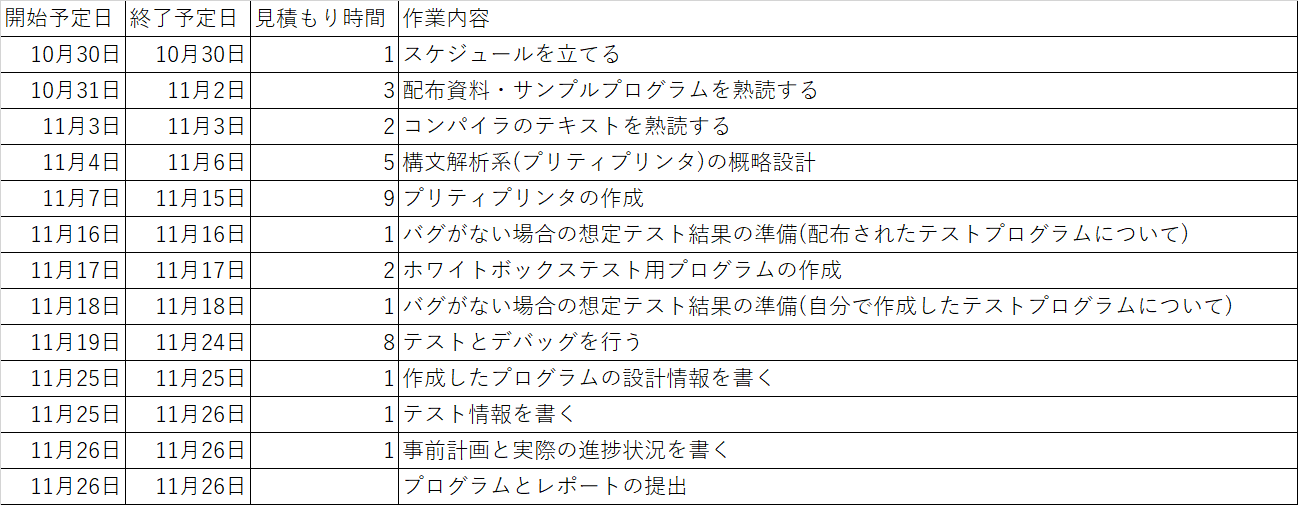
\includegraphics[scale=0.6]{kadai2-jizen.png}
\end{center}
\end{table}

しかし、演習中に計画を以下の表\ref{tb:shusei}のように修正した。
\begin{table}[H]
\begin{center}
\caption{課題2における修正後のスケジュール}
\label{tb:shusei}
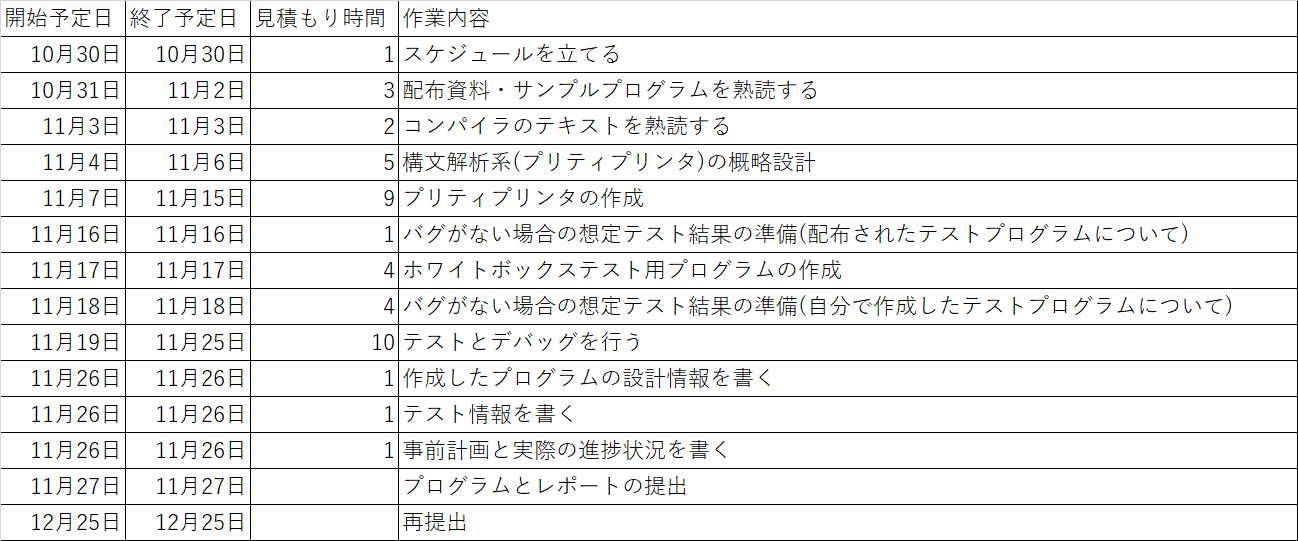
\includegraphics[scale=0.6]{kadai2-shusei.png}
\end{center}
\end{table}
\subsection{事前計画の立て方についての前課題からの改善点}
プリティプリンタのコーディングの時間を長めに確保した。
\subsection{実際の進捗状況}
表\ref{tb:shusei}のように変更したように、テストとデバッグ、特にホワイトボックステストが予想以上に時間がかかってしまった。その他の作業については
だいたい計画通りに進んだ。ただ、プログラムの最後の「.」を出力していなかったため再提出を行った。。
\subsection{当初の事前計画と実際の進捗との差の原因}
命令を網羅するために必要なテストプログラムの数の見積もりが少なかったことが原因であると考えられる。また、再提出となったのは、見直しが不十分であったからであると考えられる。
\end{document}
